%!TEX root = *.tex
%%%%%%%%%%%%%%%%%%
% カウンタのリセット
\setcounter{figure}{0}
% 問題文
図1のように,単スリット$\text{S}_0$を備えたついたてA,
複スリット$\text{S}_1$と$\text{S}_2$を備えたついたてB,
スクリーンCを平行に置き,
単色光源から出た波長$\lambda$の光を$\text{S}_0$にあてた.
光は$\text{S}_0$で回折した後,$\text{S}_1,\text{S}_2$で再び回折して,
スクリーン上に明暗の縞(干渉縞)をつくった.
$\text{S}_1$および$\text{S}_2$から等距離にあるスクリーン上の点をOとし,点Oから右に距離$x$はなれたスクリーン上の点をPとする.
$\text{S}_1$と$\text{S}_2$の間隔を$4d$,
ついたてAとついたてBの距離を$l$,
ついたてBとスクリーンCの距離を$L$,
空気の屈折率を1として,
以下の問いに答えなさい.
ただし,$l\gg 4d$,$L\gg 4d$,および$L\gg x$である.
必要であれば$\alpha\ll 1$のとき,$(1+\alpha)^\beta \fallingdotseq 1+\alpha\beta$を用いてよい.

はじめ,ついたてAは図1のように,$\text{S}_0$が$\text{S}_1$および$\text{S}_2$と等距離になる位置に置かれている.

\begin{enumerate}[(1)]
  \setlength{\leftskip}{-1.5zw}
  \setlength{\itemindent}{1zw}\setlength{\labelsep}{0.5zw}
  \setlength{\labelwidth}{1zw}\setlength{\leftmargin}{1zw}
  \setlength{\itemsep}{0.5\baselineskip}
  \item 点Pに明線が生じる条件および暗線が生じる条件をそれぞれ求めなさい.
  \item このときの明線と暗線の間隔$a$を求めよ.
\end{enumerate}

次に,図2のように,ついたてAを図の左方向に$d$だけ動かした.
この状態で干渉縞を確認すると,図1の状態で点Oにあった明線が距離$\Delta x$だけ移動していた.

\begin{enumerate}[(1)]
  \setlength{\leftskip}{-1.5zw}
  \setlength{\itemindent}{1zw}\setlength{\labelsep}{0.5zw}
  \setlength{\labelwidth}{1zw}\setlength{\leftmargin}{1zw}
  \setlength{\itemsep}{0.5\baselineskip}
  \addtocounter{enumi}{2}
  \item 明線が移動した距離$\Delta x$を求めなさい.また,移動した方向は左右どちらか答えなさい.
  \item このときの明線と暗線の間隔$b$を求めなさい.
\end{enumerate}

最後に,図3のように,ついたてAからついたてBまでの領域のうち,$\text{S}_0$から左側の領域とついたてBからスクリーンCまでの領域に,
屈折率\nn の透明な物体を置いた.
この状態で干渉縞を確認すると,図2の操作で点Oから移動した明線が点Oの位置に戻っていた.

\begin{enumerate}[(1)]
  \setlength{\leftskip}{-1.5zw}
  \setlength{\itemindent}{1zw}\setlength{\labelsep}{0.5zw}
  \setlength{\labelwidth}{1zw}\setlength{\leftmargin}{1zw}
  \setlength{\itemsep}{0.5\baselineskip}
  \addtocounter{enumi}{4}
  \item $\text{S}_0$から$\text{S}_1$を通り点Pに届く経路および$\text{S}_0$から$\text{S}_2$を通り点Pに届く経路について,光路長をそれぞれ求めなさい.
  \item 透明な物体の屈折率\nn を求めなさい.
  \item このときの明線と暗線の間隔$c$を求めなさい.
\end{enumerate}

\begin{figure}[H]
  \centering
  \begin{minipage}{.45\columnwidth}
    \centering
    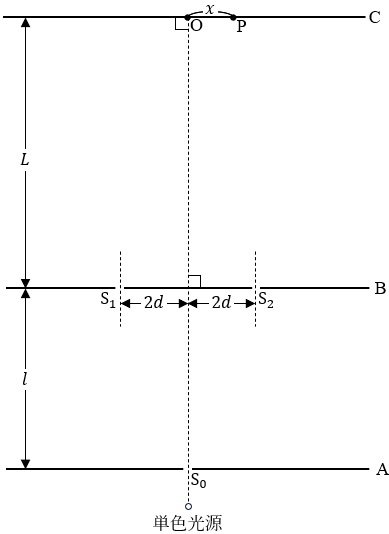
\includegraphics[width=\columnwidth]{../graphs/yokoichi_23_3-1.png}
    \caption{}
  \end{minipage}
  \begin{minipage}{.45\columnwidth}
    \centering
    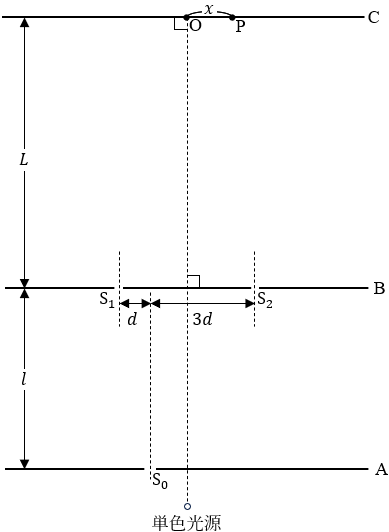
\includegraphics[width=\columnwidth]{../graphs/yokoichi_23_3-2.png}
    \caption{}
  \end{minipage}
\end{figure}
\begin{figure}[H]
  \centering
  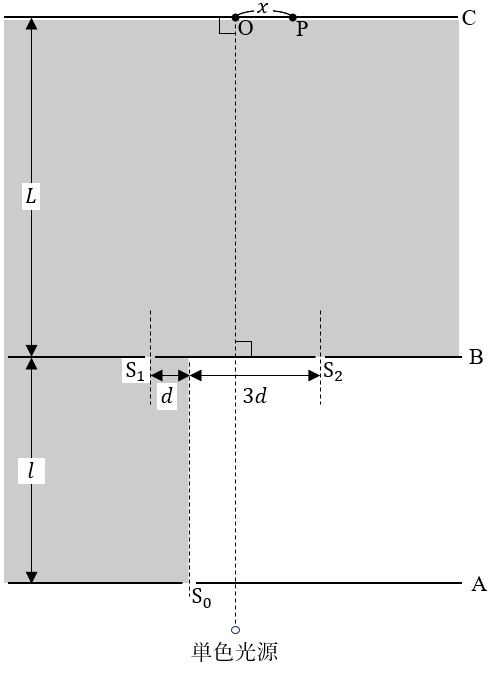
\includegraphics[width=.45\columnwidth]{../graphs/yokoichi_23_3-3.png}
  \caption{}
\end{figure}

% メモ
\begin{comment}

\end{comment}


%%%%%%%%%%%%%%%%%%
